\documentclass[12pt,a4paper]{report}

\usepackage[utf8]{inputenc}
\usepackage[margin=1in]{geometry}
\usepackage{amsmath,amssymb}
\usepackage{xcolor}
\usepackage{tikz}
\usetikzlibrary{shapes.multipart, positioning, arrows.meta, calc}
\usepackage{titlesec}
\usepackage{booktabs}
\usepackage{array}
\usepackage{tabularx}
\usepackage{hyperref}
\usepackage{fancyhdr}
\usepackage{microtype}

\hypersetup{
    colorlinks=true,
    linkcolor=black,
    urlcolor=blue!70!black,
    citecolor=black
}

% Page styling
\pagestyle{fancy}
\fancyhf{}
\lhead{\small\textsf{Heterogeneous Dynamic List (Python List in C++)}}
\rhead{}
\cfoot{\thepage}

% Title formats
\titleformat{\chapter}[display]
  {\normalfont\huge\bfseries}{\chaptertitlename\ \thechapter}{14pt}{\Huge}
\titlespacing*{\chapter}{0pt}{10pt}{20pt}

% TikZ styles for UML Diagram & Architecture
\tikzset{
    umlclass/.style={
        rectangle split,
        rectangle split parts=3,
        rectangle split part fill={white, white, white},
        draw=black,
        line width=0.8pt,
        rounded corners=2pt,
        font=\small\ttfamily,
        inner sep=6pt,
        align=left
    },
    umltrait/.style={
        rectangle split,
        rectangle split parts=2,
        rectangle split part fill={white, white},
        draw=black,
        line width=0.8pt,
        rounded corners=2pt,
        font=\small\ttfamily,
        inner sep=6pt,
        align=left
    },
    umlexception/.style={
        rectangle split,
        rectangle split parts=2,
        rectangle split part fill={white, white},
        draw=black,
        line width=0.8pt,
        rounded corners=2pt,
        font=\small\ttfamily,
        inner sep=5pt,
        align=left
    },
    inherits/.style={
        -{Triangle[open, length=8pt, width=6pt]},
        thick,
        draw=black
    },
    composition/.style={
        -{Diamond[fill=black, length=8pt, width=6pt]},
        thick,
        draw=black
    },
    dependency/.style={
        ->,
        dashed,
        thick,
        draw=black
    },
    tierframe/.style={
        draw=black,
        fill=white,
        line width=1.1pt,
        rounded corners=5pt
    },
    tierheader/.style={
        anchor=north west,
        font=\fontsize{10.5pt}{13pt}\bfseries\sffamily,
        text=black
    },
    compbox/.style={
        draw=black!75,
        fill=white,
        line width=0.7pt,
        rounded corners=3pt,
        font=\fontsize{8pt}{10pt}\sffamily,
        text=black,
        align=center,
        inner sep=4pt
    },
    flowarrow/.style={
        -{Stealth[length=6pt, width=4.5pt]},
        thick,
        draw=black
    },
    dasharrow/.style={
        -{Stealth[length=6pt, width=4.5pt]},
        dashed,
        thick,
        draw=black
    }
}

\begin{document}

% Configure numbering to start at Chapter 21 (all sections 21.x, tables 21.x, figures 21.x)
\setcounter{chapter}{20}

\chapter{Heterogeneous Dynamic List (Python List in C++)}
\setcounter{chapter}{21}
\renewcommand{\thechapter}{21}
\renewcommand{\thesection}{21.\arabic{section}}
\renewcommand{\thesubsection}{21.\arabic{section}.\arabic{subsection}}
\renewcommand{\thetable}{21.\arabic{table}}
\renewcommand{\thefigure}{21.\arabic{figure}}
\textbf{Authors:} Akhshay Arulpragasam, Jeevan R

\vspace{1.5em}

\section{Introduction and Problem Statement}

Python's built-in \texttt{list} is one of the most versatile and ubiquitous dynamic data structures in modern software engineering. It allows values of arbitrary types---integers, floating-point numbers, strings, nested lists, and user-defined structures---to coexist within a single, dynamically resizable container. Everyday operations such as negative indexing, multi-step slicing, element removal by value, and list concatenation are standard idioms in Python.

C++, in contrast, enforces strict compile-time type homogeneity across its standard container suite. A \texttt{std::vector<int>} can hold only integers; a \texttt{std::vector<std::string>} can hold only strings. Standard C++ provides no native container that simultaneously stores \texttt{int}, \texttt{double}, \texttt{std::string}, and user-defined classes without resorting to invasive base-class inheritance hierarchies, type-erased \texttt{void*} pointers coupled with manual heap allocations, or closed static unions like \texttt{std::variant} which require all types to be enumerated at compile-time.

\textbf{Problem Statement:} Design and implement a robust C++17 library that provides a Python-style heterogeneous dynamic list container. The system must allow elements of arbitrary data types---integers, floats, strings, and nested lists---to coexist dynamically within the same container. The implementation requires:
\begin{enumerate}
    \item Modern type erasure using \texttt{std::any} rather than error-prone \texttt{void*} pointers or manual memory management.
    \item Deep operator overloading (\texttt{operator[]}, \texttt{operator+}, \texttt{operator+=}, and \texttt{operator<<}).
    \item Nested class structures (\texttt{ProxyElement}) facilitating transparent type access, implicit conversion, and stream redirection.
    \item Pythonic semantics emulation including signed negative indexing, arbitrary step slicing with boundary clamping, and copy/reference value semantics.
    \item Comprehensive exception handling for type extraction mismatches, invalid boundaries, and unsupported operations.
\end{enumerate}

From an end-user perspective, the library exposes a unified \texttt{PythonList} interface through a standard header include (\texttt{\#include <PythonList>}). Developers can append elements of any type, access elements using negative offsets (\texttt{list[-1]}), extract typed values implicitly (\texttt{int x = list[0]}) or explicitly (\texttt{list[0].getValue<int>()}), remove elements by value, slice sub-lists, concatenate containers, and stream the entire collection directly to \texttt{std::cout} without dealing with the underlying \texttt{std::any} casting machinery.

\section{Scope and Feature Set}

The system provides the following comprehensive capabilities:

\begin{itemize}
    \item \textbf{Heterogeneous Storage via Type Erasure:} Stored elements reside in a unified contiguous dynamic array (\texttt{std::vector<std::any>}). Any type meeting \texttt{std::any}'s copy-constructible requirements can be stored without pre-registering permitted types.
    
    \item \textbf{C-String Normalization:} Specialized overloads for \texttt{const char*} automatically convert string literals into \texttt{std::string} instances upon insertion, preventing dangling pointer bugs and lifecycle mismatches.
    
    \item \textbf{Transparent Proxy-Based Element Access (\texttt{ProxyElement}):} The subscript operator returns a nested \texttt{ProxyElement} bridge holding an internal reference to the targeted \texttt{std::any}. This proxy supports implicit type deduction via a templated \texttt{operator T()}, explicit extraction via \texttt{getValue<T>()}, and stream output redirection via \texttt{print()}.
    
    \item \textbf{Value and Reference Storage Semantics:} Value semantics are preserved by default using move and copy construction. In addition, the \texttt{appendReference()} method enables storing \texttt{std::reference\_wrapper<T>} instances, allowing modifications in the list to reflect directly in the caller's referenced external object.
    
    \item \textbf{Negative Indexing:} Every indexing method (\texttt{operator[]}, \texttt{insert}, and \texttt{pop}) supports Python-style signed negative indices (where \texttt{-1} accesses the last element, \texttt{-2} accesses the second to last), with bounds validation throwing \texttt{std::out\_of\_range}.
    
    \item \textbf{Insertion and Removal Operations:} The \texttt{insert()} method inserts elements at arbitrary positions with Python-standard index clamping (out-of-bound indices clamp to list boundaries rather than throwing). The \texttt{pop()} method removes and returns elements by index (defaulting to the tail). The \texttt{remove()} method removes the first element matching both type and equality, while \texttt{contains()} performs non-destructive membership verification.
    
    \item \textbf{Concatenation and Extension:} Lists can be extended in place using \texttt{extend()} or \texttt{operator+=}, and concatenated non-destructively using \texttt{operator+}. Self-extension is handled safely.
    
    \item \textbf{Multi-Directional Slicing:} The \texttt{slice(start, stop, step)} method extracts sub-lists with arbitrary positive or negative step strides and index clamping. Non-valid step sizes (\texttt{step == 0}) throw \texttt{std::invalid\_argument}.
    
    \item \textbf{Dynamic Polymorphic Printing:} A static function registry mapping each \texttt{std::type\_\allowbreak index} to dynamic printer closures via \texttt{std::un\-or\-dered\_\allowbreak map}. The \texttt{operator<<} overload prints Python-like bracketed lists (\texttt{[10, 3.14, Hello]}).
    
    \item \textbf{Domain-Specific Exception Hierarchy:} Custom exceptions derived from \texttt{std::run\-time\_\allowbreak error} (\texttt{Type\-Mis\-match\-Er\-ror}, \texttt{Un\-sup\-port\-ed\-Op\-er\-a\-tion\-Er\-ror}, and \texttt{Ar\-gu\-ment\-Not\-Pre\-sent\-Er\-ror}) deliver clear diagnostic messages while isolating callers from standard runtime internals.
    
    \item \textbf{Modern CMake Integration:} Full packaging support with CMake target exports (\texttt{PythonList::PythonList}), \texttt{GNUInstallDirs} installation rules, and CTest-integrated regression test suites.
\end{itemize}

\newpage
\section{Object-Oriented Architecture}

The system addresses the fundamental challenge of runtime type dynamicity in a statically typed language by coordinating core Object-Oriented Programming (OOP) principles and compile-time metaprogramming:

\begin{itemize}
    \item \textbf{Encapsulation:} The internal data structure (\texttt{std::vector<std::any>}) and the static printing lookup table are completely private to \texttt{PythonList}. All interactions occur via public member functions and operator overloads, insulating consumer code from underlying implementation details.
    
    \item \textbf{Abstraction via the Proxy Pattern:} Direct indexing into a heterogeneous container cannot have a single compile-time return type. \texttt{ProxyElement} abstracts this limitation by functioning as an intermediary evaluator that delays and infers type casting at the assignment site.
    
    \item \textbf{Inheritance:} The custom exception classes (\texttt{Type\-Mis\-match\-Er\-ror}, \texttt{Un\-sup\-port\-ed\-Op\-er\-a\-tion\-Er\-ror}, and \texttt{Ar\-gu\-ment\-Not\-Pre\-sent\-Er\-ror}) inherit directly from \texttt{std::run\-time\_\allowbreak error}, integrating cleanly into standard C++ exception handling pipelines.
    
    \item \textbf{Compile-Time Metaprogramming (SFINAE):} The type traits \texttt{IsPrintable<T>} and \texttt{IsEqualityComparable<T>} use \texttt{std::void\_t} and \texttt{if constexpr} to conditionally inspect and enforce type capabilities at compile time without generating template instantiation errors.
    
    \item \textbf{Deep Operator Overloading:} The library overloads \texttt{operator[]}, \texttt{operator+}, \texttt{operator+=}, and \texttt{operator<<} for both \texttt{PythonList} and \texttt{ProxyElement}, providing intuitive, Pythonic syntax.
\end{itemize}

\subsection{Class Design and Associations}

The primary components and structural associations in the codebase are detailed below:

\begin{enumerate}
    \item \textbf{\texttt{PythonList} (Container Engine):} Manages the contiguous array of type-erased elements and registers printing functions.
    \item \textbf{\texttt{PythonList::ProxyElement} (Inner Proxy Class -- Composition):} Defined as a public nested class within \texttt{PythonList}. It maintains a \texttt{std::any\&} reference to the indexed list element and provides lazy extraction methods (\texttt{getValue<T>()}, \texttt{operator T()}, \texttt{print()}). It cannot exist independently of the referenced container element.
    \item \textbf{Exception Hierarchy (Inheritance):}
    \begin{itemize}
        \item \texttt{TypeMismatchError}: Thrown when extracting an element into an incompatible type.
        \item \texttt{UnsupportedOperationError}: Thrown when performing equality-dependent operations (\texttt{remove}, \texttt{contains}) on types lacking \texttt{operator==}.
        \item \texttt{ArgumentNotPresentError}: Thrown when \texttt{remove()} fails to locate the specified value.
    \end{itemize}
    \item \textbf{Compile-Time Type Traits (Dependencies):}
    \begin{itemize}
        \item \texttt{IsPrintable<T, void>}: SFINAE trait detecting if stream insertion (\texttt{std::ostream << T}) is defined.
        \item \texttt{IsEqualityComparable<T, void>}: SFINAE trait verifying whether \texttt{operator==} is supported.
    \end{itemize}
\end{enumerate}

\begin{table}[htbp]
\centering
\small
\begin{tabularx}{\linewidth}{@{} >{\raggedright\arraybackslash}p{3.5cm} >{\raggedright\arraybackslash}p{2.6cm} >{\raggedright\arraybackslash}p{2.2cm} X@{}}
\toprule
\textbf{Source Entity} & \textbf{Target Entity} & \textbf{Relationship} & \textbf{Architectural Description} \\
\midrule
\texttt{PythonList} & \texttt{ProxyElement} & Composition & Nested inner class instantiated and returned by \texttt{operator[]}. \\
\texttt{TypeMismatchError} & \texttt{std::run\-time\_\allowbreak error} & Inheritance & Derives standard error reporting and \texttt{what()} interface. \\
\texttt{Un\-sup\-port\-ed\-Op\-er\-a\-tion\-Er\-ror} & \texttt{std::run\-time\_\allowbreak error} & Inheritance & Derives standard error reporting and \texttt{what()} interface. \\
\texttt{Ar\-gu\-ment\-Not\-Pre\-sent\-Er\-ror} & \texttt{std::run\-time\_\allowbreak error} & Inheritance & Derives standard error reporting and \texttt{what()} interface. \\
\texttt{PythonList} & \texttt{IsPrintable<T>} & Dependency & Compile-time validation prior to printer registration. \\
\texttt{PythonList} & \texttt{IsEquality-}\\\texttt{Comparable<T>} & Dependency & Compile-time validation prior to equality evaluation. \\
\bottomrule
\end{tabularx}
\caption{Structural Relationships and Associations in \texttt{include/List.h}.}
\label{tab:associations}
\end{table}

\newpage
\subsection{UML Class Diagram}

The complete UML Class Diagram representing all entities, members, types, and associations declared in \texttt{include/List.h} is illustrated in Figure~\ref{fig:uml_class}.

\begin{figure}[htbp]
\centering
\resizebox{0.95\textwidth}{!}{
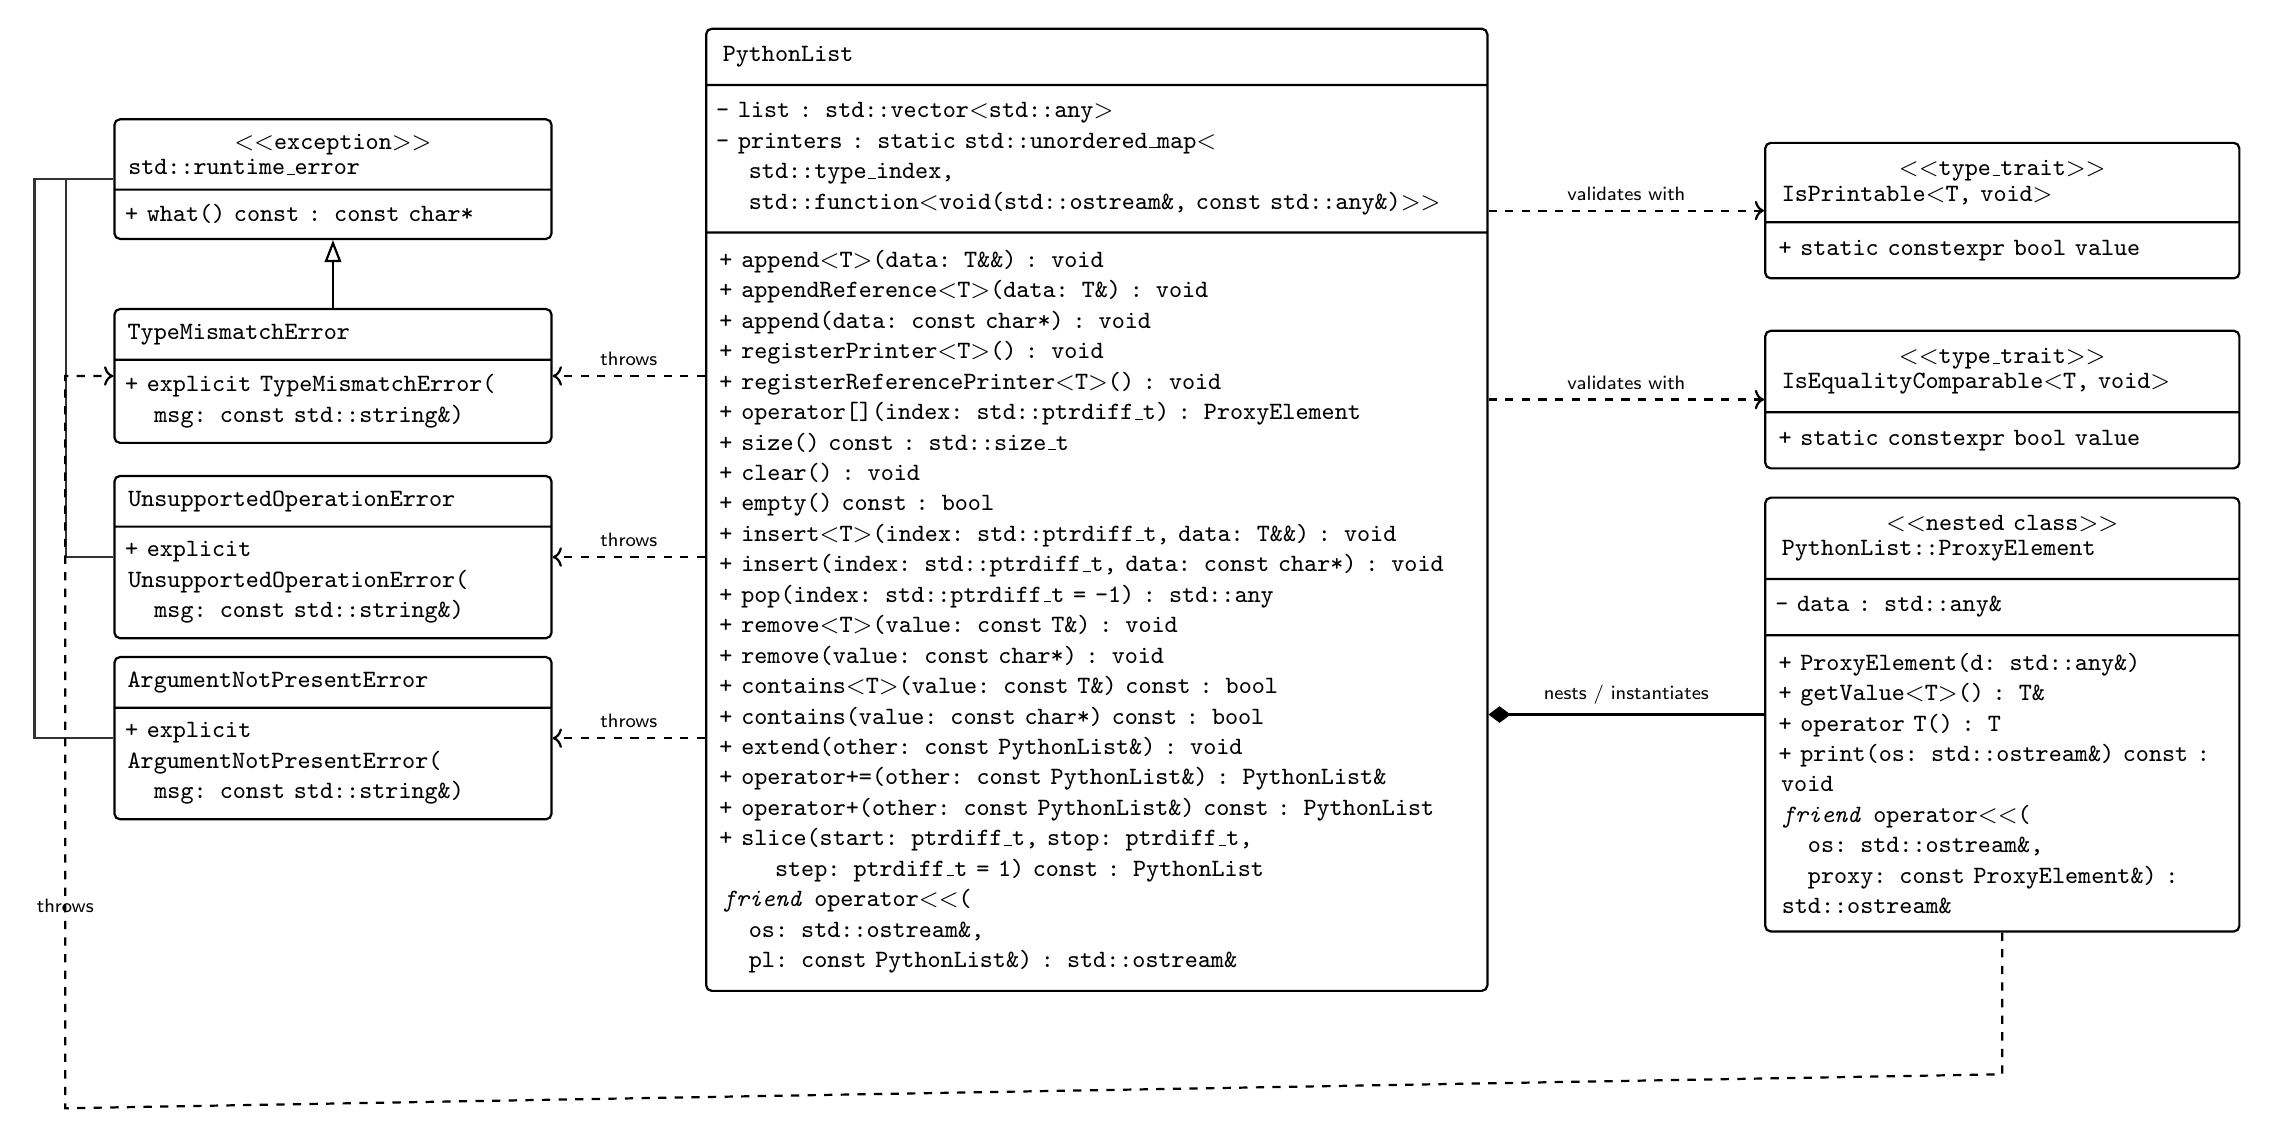
\begin{tikzpicture}[auto]

    % COLUMN 1 (LEFT): EXCEPTION HIERARCHY
    \node (runtime_error) [umlexception, text width=5.2cm] at (-9.2, 4.8) {
        \centering\textbf{\textless\textless exception\textgreater\textgreater}\\[-0.2em]
        \centering\textbf{std::runtime\_error}
        \nodepart{second}
        + what() const : const char*
    };

    \node (type_mismatch) [umlexception, text width=5.2cm] at (-9.2, 2.3) {
        \centering\textbf{TypeMismatchError}
        \nodepart{second}
        + explicit TypeMismatchError(\\
        \quad msg: const std::string\&)
    };

    \node (unsupported_op) [umlexception, text width=5.2cm] at (-9.2, 0.0) {
        \centering\textbf{UnsupportedOperationError}
        \nodepart{second}
        + explicit UnsupportedOperationError(\\
        \quad msg: const std::string\&)
    };

    \node (arg_not_present) [umlexception, text width=5.2cm] at (-9.2, -2.3) {
        \centering\textbf{ArgumentNotPresentError}
        \nodepart{second}
        + explicit ArgumentNotPresentError(\\
        \quad msg: const std::string\&)
    };

    % Inheritance
    \draw [inherits] (type_mismatch.north) -- (runtime_error.south);
    \draw [thick, draw=black!80] (unsupported_op.west) -- ++(-0.6, 0) |- (runtime_error.west);
    \draw [thick, draw=black!80] (arg_not_present.west) -- ++(-1.0, 0) |- (runtime_error.west);

    % COLUMN 2 (CENTER): MAIN CONTAINER PythonList
    \node (python_list) [umlclass, text width=9.5cm] at (0.5, 0.6) {
        \centering\textbf{PythonList}
        \nodepart{second}
        - list : std::vector\textless std::any\textgreater \\
        - printers : static std::unordered\_map\textless\\
        \quad std::type\_index,\\
        \quad std::function\textless void(std::ostream\&, const std::any\&)\textgreater\textgreater
        \nodepart{third}
        + append\textless T\textgreater(data: T\&\&) : void\\
        + appendReference\textless T\textgreater(data: T\&) : void\\
        + append(data: const char*) : void\\
        + registerPrinter\textless T\textgreater() : void\\
        + registerReferencePrinter\textless T\textgreater() : void\\
        + operator[](index: std::ptrdiff\_t) : ProxyElement\\
        + size() const : std::size\_t\\
        + clear() : void\\
        + empty() const : bool\\
        + insert\textless T\textgreater(index: std::ptrdiff\_t, data: T\&\&) : void\\
        + insert(index: std::ptrdiff\_t, data: const char*) : void\\
        + pop(index: std::ptrdiff\_t = -1) : std::any\\
        + remove\textless T\textgreater(value: const T\&) : void\\
        + remove(value: const char*) : void\\
        + contains\textless T\textgreater(value: const T\&) const : bool\\
        + contains(value: const char*) const : bool\\
        + extend(other: const PythonList\&) : void\\
        + operator+=(other: const PythonList\&) : PythonList\&\\
        + operator+(other: const PythonList\&) const : PythonList\\
        + slice(start: ptrdiff\_t, stop: ptrdiff\_t,\\
        \quad\quad step: ptrdiff\_t = 1) const : PythonList\\
        \textit{friend} operator\textless\textless(\\
        \quad os: std::ostream\&,\\
        \quad pl: const PythonList\&) : std::ostream\&
    };

    % COLUMN 3 (RIGHT): TRAITS & PROXY ELEMENT
    \node (is_printable) [umltrait, text width=5.6cm] at (12.0, 4.4) {
        \centering\textbf{\textless\textless type\_trait\textgreater\textgreater}\\[-0.2em]
        \centering\textbf{IsPrintable\textless T, void\textgreater}
        \nodepart{second}
        + static constexpr bool value
    };

    \node (is_equality) [umltrait, text width=5.6cm] at (12.0, 2.0) {
        \centering\textbf{\textless\textless type\_trait\textgreater\textgreater}\\[-0.2em]
        \centering\textbf{IsEqualityComparable\textless T, void\textgreater}
        \nodepart{second}
        + static constexpr bool value
    };

    \node (proxy_element) [umlclass, text width=5.6cm] at (12.0, -2.0) {
        \centering\textbf{\textless\textless nested class\textgreater\textgreater}\\[-0.2em]
        \centering\textbf{PythonList::ProxyElement}
        \nodepart{second}
        - data : std::any\&
        \nodepart{third}
        + ProxyElement(d: std::any\&)\\
        + getValue\textless T\textgreater() : T\&\\
        + operator T() : T\\
        + print(os: std::ostream\&) const : void\\
        \textit{friend} operator\textless\textless(\\
        \quad os: std::ostream\&,\\
        \quad proxy: const ProxyElement\&) : std::ostream\&
    };

    % Relationships
    \draw [dependency] (python_list.west |- type_mismatch.east) -- 
          node[above, midway, font=\scriptsize\sffamily] {throws} (type_mismatch.east);

    \draw [dependency] (python_list.west |- unsupported_op.east) -- 
          node[above, midway, font=\scriptsize\sffamily] {throws} (unsupported_op.east);

    \draw [dependency] (python_list.west |- arg_not_present.east) -- 
          node[above, midway, font=\scriptsize\sffamily] {throws} (arg_not_present.east);

    \draw [dependency] (python_list.east |- is_printable.west) -- 
          node[above, midway, font=\scriptsize\sffamily] {validates with} (is_printable.west);

    \draw [dependency] (python_list.east |- is_equality.west) -- 
          node[above, midway, font=\scriptsize\sffamily] {validates with} (is_equality.west);

    \draw [composition] (proxy_element.west) -- 
          node[above, midway, font=\scriptsize\sffamily] {nests / instantiates} (python_list.east |- proxy_element.west);

    \draw [dependency] (proxy_element.south) -- ++(0, -1.8) -- (-12.6, -7.0) |- 
          node[pos=0.15, below, font=\scriptsize\sffamily] {throws} (type_mismatch.west);

\end{tikzpicture}
}
\caption{UML Class Diagram of \texttt{include/List.h}.}
\label{fig:uml_class}
\end{figure}

\newpage
\subsection{System Architecture Blueprint}

The end-to-end layered architecture mapping the operating environment, public API, dynamic dispatch registry, storage core, exception subsystem, and CMake pipeline is illustrated in Figure~\ref{fig:arch_blueprint}.

\begin{figure}[htbp]
\centering
\resizebox{\textwidth}{!}{
\begin{tikzpicture}

    % =========================================================================
    % TIER 1: CLIENT & OPERATING ENVIRONMENT
    % =========================================================================
    \draw [tierframe] (-10.0, 7.8) rectangle (10.0, 10.9);
    \node [tierheader] at (-9.6, 10.65) 
          {1. Operating Environment \& Consumer Layer};

    \node (app) [compbox, text width=5.8cm] at (-6.4, 8.9) {
        \textbf{User Application Target}\\
        \texttt{main.cpp}\\
        {\scriptsize High-level heterogeneous container usage}
    };

    \node (tests) [compbox, text width=5.8cm] at (0.0, 8.9) {
        \textbf{CTest Regression Test Suites}\\
        \texttt{tests/regression\_test.cpp}, \texttt{P1test}, \texttt{P2test}\\
        {\scriptsize Full Phase 1 \& Phase 2 validation}
    };

    \node (wrapper) [compbox, text width=5.8cm] at (6.4, 8.9) {
        \textbf{Public Standard Header Facade}\\
        \texttt{include/PythonList} $\rightarrow$ \texttt{include/List.h}\\
        {\scriptsize Canonical extensionless include facade}
    };

    \draw [flowarrow] (app.east) -- (tests.west);
    \draw [flowarrow] (tests.east) -- (wrapper.west);

    % =========================================================================
    % TIER 2: PUBLIC INTERFACE & PROXY TIER
    % =========================================================================
    \draw [tierframe] (-10.0, 3.5) rectangle (10.0, 7.2);
    \node [tierheader] at (-9.6, 6.95) 
          {2. Public Interface \& Transparent Proxy Layer (\texttt{include/List.h}, \texttt{src/List.cpp})};

    \node (mutators) [compbox, text width=4.3cm] at (-7.35, 4.9) {
        \textbf{Mutation Engine}\\
        \texttt{append(T\&\&)}, \texttt{insert(idx, T)}\\
        \texttt{pop(idx)}, \texttt{remove(val)}\\
        \texttt{clear()}, \texttt{extend(other)}
    };

    \node (queries) [compbox, text width=4.3cm] at (-2.45, 4.9) {
        \textbf{Query \& Slice Engine}\\
        \texttt{size()}, \texttt{empty()}, \texttt{contains()}\\
        \texttt{slice(start, stop, step)}\\
        {\scriptsize Clamping \& negative step handling}
    };

    \node (operators) [compbox, text width=4.3cm] at (2.45, 4.9) {
        \textbf{Operator Overloads}\\
        \texttt{operator+=(other)}\\
        \texttt{operator+(other)}\\
        \texttt{operator\textless\textless(ostream\&, pl)}
    };

    \node (proxy) [compbox, text width=4.3cm] at (7.35, 4.9) {
        \textbf{ProxyElement Bridge}\\
        \texttt{operator[](ptrdiff\_t)}\\
        \texttt{operator T()} {\scriptsize (implicit cast)}\\
        \texttt{getValue\textless T\textgreater()} {\scriptsize (explicit cast)}
    };

    \draw [flowarrow] (mutators.east) -- (queries.west);
    \draw [flowarrow] (queries.east) -- (operators.west);
    \draw [flowarrow] (operators.east) -- (proxy.west);

    % =========================================================================
    % TIER 3: METAPROGRAMMING & DYNAMIC DISPATCH ENGINE
    % =========================================================================
    \draw [tierframe] (-10.0, -0.6) rectangle (10.0, 2.9);
    \node [tierheader] at (-9.6, 2.65) 
          {3. Metaprogramming Introspection \& Dynamic Dispatch Engine};

    \node (sfinae_print) [compbox, text width=4.3cm] at (-7.35, 0.8) {
        \textbf{SFINAE: \texttt{IsPrintable\textless T\textgreater}}\\
        \texttt{std::void\_t} detection\\
        {\scriptsize Validates \texttt{ostream \textless\textless\ const T\&}}
    };

    \node (sfinae_eq) [compbox, text width=4.3cm] at (-2.45, 0.8) {
        \textbf{SFINAE: \texttt{IsEqualityComparable}}\\
        \texttt{operator==} compile check\\
        {\scriptsize Guards \texttt{contains()} and \texttt{remove()}}
    };

    \node (jit_printer) [compbox, text width=4.3cm] at (2.45, 0.8) {
        \textbf{JIT Printer Registration}\\
        \texttt{registerPrinter\textless T\textgreater()}\\
        \texttt{registerReferencePrinter\textless T\textgreater()}\\
        {\scriptsize Generates closure on element insert}
    };

    \node (printer_map) [compbox, text width=4.3cm] at (7.35, 0.8) {
        \textbf{Static Type Registry}\\
        \texttt{unordered\_map\textless type\_index,}\\
        \texttt{function\textless void(os\&, any\&)\textgreater\textgreater}\\
        {\scriptsize $O(1)$ runtime polymorphic streaming}
    };

    \draw [dasharrow] (sfinae_print.east) -- (sfinae_eq.west);
    \draw [flowarrow] (sfinae_eq.east) -- (jit_printer.west);
    \draw [flowarrow] (jit_printer.east) -- (printer_map.west);

    % =========================================================================
    % TIER 4: HETEROGENEOUS STORAGE CORE
    % =========================================================================
    \draw [tierframe] (-10.0, -4.7) rectangle (10.0, -1.2);
    \node [tierheader] at (-9.6, -1.45) 
          {4. Type-Erased Heterogeneous Storage Engine Core};

    \node (vec_storage) [compbox, text width=4.3cm] at (-7.35, -3.3) {
        \textbf{Contiguous Vector}\\
        \texttt{std::vector\textless std::any\textgreater\ list}\\
        {\scriptsize Small Buffer Optimization (SBO)}
    };

    \node (val_semantics) [compbox, text width=4.3cm] at (-2.45, -3.3) {
        \textbf{Value Semantics}\\
        Primitive scalars, strings, structs\\
        {\scriptsize Stored by value in \texttt{std::any}}
    };

    \node (ref_semantics) [compbox, text width=4.3cm] at (2.45, -3.3) {
        \textbf{Reference Semantics}\\
        \texttt{appendReference(T\&)}\\
        {\scriptsize Stored in \texttt{std::reference\_wrapper}}
    };

    \node (cstring_decay) [compbox, text width=4.3cm] at (7.35, -3.3) {
        \textbf{String Specialization}\\
        \texttt{const char*} overloads\\
        {\scriptsize Auto-decay to \texttt{std::string}}
    };

    \draw [flowarrow] (vec_storage.east) -- (val_semantics.west);
    \draw [flowarrow] (val_semantics.east) -- (ref_semantics.west);
    \draw [flowarrow] (ref_semantics.east) -- (cstring_decay.west);

    % =========================================================================
    % TIER 5: SAFETY SUBSYSTEM (BOTTOM LEFT)
    % =========================================================================
    \draw [tierframe] (-10.0, -9.5) rectangle (-0.3, -5.3);
    \node [tierheader] at (-9.6, -5.55) 
          {5. Safety \& Domain Exception Subsystem};

    \node (custom_err) [compbox, text width=8.9cm] at (-5.15, -6.9) {
        \textbf{Custom Domain Exceptions (inherit \texttt{std::runtime\_error})}\\
        \texttt{TypeMismatchError} \enspace\textbullet\enspace
        \texttt{UnsupportedOperationError} \enspace\textbullet\enspace
        \texttt{ArgumentNotPresentError}
    };

    \node (std_err) [compbox, text width=8.9cm] at (-5.15, -8.5) {
        \textbf{Standard Boundary \& Step Exceptions}\\
        \texttt{std::out\_of\_range} (invalid index) \enspace\textbullet\enspace
        \texttt{std::invalid\_argument} (slice step == 0)
    };

    % =========================================================================
    % TIER 6: BUILD & DISTRIBUTION (BOTTOM RIGHT)
    % =========================================================================
    \draw [tierframe] (0.3, -9.5) rectangle (10.0, -5.3);
    \node [tierheader] at (0.7, -5.55) 
          {6. Build, Packaging \& Distribution Pipeline};

    \node (cmake_box) [compbox, text width=8.9cm] at (5.15, -6.9) {
        \textbf{Modern CMake Build Configuration}\\
        \texttt{CMakeLists.txt} (\texttt{cxx\_std\_17}) \enspace\textbullet\enspace
        Target: \texttt{PythonList} \enspace\textbullet\enspace
        \texttt{BUILD\_INTERFACE}
    };

    \node (pkg_box) [compbox, text width=8.9cm] at (5.15, -8.5) {
        \textbf{Package Export \& Test Execution}\\
        \texttt{cmake/PythonListConfig.cmake.in} \enspace\textbullet\enspace
        \texttt{GNUInstallDirs} \enspace\textbullet\enspace
        CTest Runner
    };

    % =========================================================================
    % VERTICAL PIPELINE ARROWS (CENTER CHANNEL - ZERO OVERLAPS)
    % =========================================================================
    \draw [flowarrow] (0, 7.8) -- node[right, font=\scriptsize\sffamily, text=black] {invokes API} (0, 7.2);
    \draw [flowarrow] (0, 3.5) -- node[right, font=\scriptsize\sffamily, text=black] {validates \& registers} (0, 2.9);
    \draw [flowarrow] (0, -0.6) -- node[right, font=\scriptsize\sffamily, text=black] {stores erased types} (0, -1.2);

    % =========================================================================
    % OUTER PERIMETER CONNECTORS (STRICTLY OUTSIDE ALL BOXES - ZERO OVERLAPS)
    % =========================================================================
    % Outer left connector: Tier 2 -> Tier 5 (Throws on error)
    \draw [dasharrow] (-10.0, 5.0) -- ++(-0.8, 0) |- 
          node[pos=0.25, left, font=\scriptsize\sffamily, text=black] {throws on error} (-10.0, -7.4);

    % Outer right connector: Tier 6 -> Tier 1 (Compiles and tests)
    \draw [dasharrow] (10.0, -7.4) -- ++(0.8, 0) |- 
          node[pos=0.25, right, font=\scriptsize\sffamily, text=black] {compiles \& verifies} (10.0, 8.9);

\end{tikzpicture}
}
\caption{System Architecture Blueprint of the Heterogeneous Dynamic List Container.}
\label{fig:arch_blueprint}
\end{figure}

\newpage
\section{Technology Stack}

The Heterogeneous Dynamic List library is engineered using modern ISO C++ standards, declarative build configurations, and formal verification harnesses to ensure compile-time type safety, deterministic destruction, and seamless developer ergonomics. Table~\ref{tab:tech_stack} details the complete toolchain and technology stack powering the project.

\begin{table}[htbp]
\centering
\small
\begin{tabularx}{\linewidth}{@{} >{\raggedright\arraybackslash}p{3.2cm} >{\raggedright\arraybackslash}p{3.8cm} X@{}}
\toprule
\textbf{Component Layer} & \textbf{Technology / Tool} & \textbf{Architectural Role \& Utilization} \\
\midrule
\textbf{Programming Language} & ISO Modern C++17 \newline (\texttt{-std=c++17}) & Core container language utilizing modern features including \texttt{std::any}, \texttt{std::void\_t}, structured bindings, and fold expressions. \\
\addlinespace
\textbf{Type Erasure Core} & \texttt{std::any} \& \newline \texttt{std::type\_index} & Dynamic homogeneous array abstraction allowing arbitrary copy-constructible objects to reside in a contiguous memory block without inheritance. \\
\addlinespace
\textbf{Metaprogramming} & SFINAE \& \newline \texttt{if constexpr} & Compile-time type introspection (\texttt{IsPrintable}, \texttt{IsEqualityComparable}) to conditionally guard member functions and printer registration. \\
\addlinespace
\textbf{Memory Semantics} & \texttt{std::vector}, \newline \texttt{reference\_wrapper} & RAII-compliant automatic lifecycle management with Small Buffer Optimization (SBO) and support for explicit reference semantics. \\
\addlinespace
\textbf{Build \& Packaging} & Modern CMake \newline (\texttt{v3.15+}) & Modular cross-platform compilation, target export (\texttt{PythonList::PythonList}), and installation rules via \texttt{GNUInstallDirs}. \\
\addlinespace
\textbf{Test Framework} & CTest \& \newline Custom Harnesses & Automated regression suites, edge-case boundary testing, signed negative indexing assertions, and memory integrity verification. \\
\addlinespace
\textbf{Documentation} & \LaTeX{} (Report) \& \newline TikZ/PGF & Production of publication-quality formal specifications, UML class diagrams, and multi-tier architectural blueprints. \\
\bottomrule
\end{tabularx}
\caption{Comprehensive Technology Stack and Toolchain Specifications.}
\label{tab:tech_stack}
\end{table}

\subsection{Toolchain and Environmental Requirements}
\begin{itemize}
    \item \textbf{C++ Compiler:} GCC 9+, Clang 10+, or Microsoft Visual Studio 2019+ with complete C++17 standard library support.
    \item \textbf{Build Tool:} CMake version 3.15 or newer with Ninja or GNU Make generators.
    \item \textbf{Memory Model:} Deterministic stack and heap resource acquisition using modern RAII paradigms; zero raw pointer ownership.
    \item \textbf{Operating Environments:} Multi-platform support validated on Linux (Ubuntu 20.04/22.04 LTS), macOS, and Windows 10/11 (MSVC/MinGW).
\end{itemize}

\end{document}
